\chapter{Biblioteka: Take Me Home}
\label{app:takeMeHome}
\thispagestyle{appendixStyle}





Wszystkie algorytmy, które wcześniej opisywaliśmy, zostały zaimplementowane w języku $C$ (standard $C99$) i~umieszczone w bibliotece o~przewrotnie nazwanej \textit{Take Me Home} (jako, że wszystkie algorytmy miały za zadanie wyszukiwanie najkrótszych ścieżek).
W~niniejszym rozdziale omówimy strukturę wykorzystanej biblioteki, skupiając się na jej kluczowych własnościach i~operacjach które za jej pomocą wykonamy.
Przyjrzymy się udostępnionemu użytkownikowi interfejsie oraz prześledzimy przykładową sesję działania prostego programu wykorzystującego tą bibliotekę.




\section{Wymagania i~instalacja}




Biblioteka w całości została napisana w języku programowania \textsc{C} (zgodnie z~jego wszystkimi standardami ustalonymi przez \textit{\textsc{ISO 9899:1999}}) na komputerze pracującym pod kontrolą systemu \textsc{Ubuntu 14.04.1 LTS} dla architektury \textsc{64}-bitowej.
W~związku z~tym wszystkie skrypty, które będą opisywane w poniższych podrozdziałach, oraz przykłady wywołań owych programów będą specyficzne dla tego systemu operacyjnego.
Co za tym idzie, aby wykorzystać bibliotekę na komputerze pod kontrolą innego systemu operacyjnego, niezbędne może okazać się przystosowanie biblioteki pod dany system, dlatego też wraz ze skompilowaną wersją biblioteki są też udostępnione jej wszystkie kody źródłowe wraz z~przykładowym programem mającym na celu zweryfikować poprawność jej działania.
W~związku z~tym, poniżej został przedstawiony cały proces kompilacji biblioteki aż do momentu uruchomienia testowego programu, który ją wykorzystuje.

Struktura katalogów wszystkich plików, wchodzących w skład biblioteki wygląda następująco:

\dirtree{%
.1 /.
.2 \textsc{\textcolor{lgray}{Presentations}}.
.2 \textsc{\textcolor{lgray}{References}}.
.2 \textsc{Scripts}.
.2 \textsc{\textcolor{lgray}{Thesis}}.
.2 \textsc{TMH\_Examples}.
.2 \textsc{TMH\_Library}.
.2 \textsc{TMH\_GraphHelper}.
.2 clear.bash. 
.2 README.md. 
}

Katalogi, które zostały wyszarzone nie interesują nas z~punktu widzenia implementacji biblioteki.
W~pozostałych katalogach znajdują się odpowiednio kody źródłowe odpowiadające za dane części funkcjonalności, które oddają ich nazwy.
Aby skompilować oba projekty naraz, należy wykorzystać skrypt znajdujący się w odpowiednim katalogu: \textsf{/Scripts/compileProject.bash}, uruchamiając go poleceniem wpisanym w terminalu (\texttt{CRTL + ALT + T}):

\begin{lstlisting}[language=bash]
pcname@user:/Scripts$ bash compileProject.bash
\end{lstlisting}

\small
\begin{lstlisting}[language=bash]
----------------------------------------------------
Enter full path to library project or leave empty (TMH_Library/):
Enter full path to sample project or leave empty (TMH_Examples/):
Enter full path for where generated library should be copy or leave empty (/usr/lib):
Enter name for generated program or leave empty (run):
...
\end{lstlisting}
\normalsize

Nim proces kompilacji się rozpocznie, zostaniemy poproszeniu o~podanie dodatkowych informacji.
W~przypadku pozostawienia pustych linii zostaną ustawione domyślne wartości podane w~nawiasach (zgodne z~oryginalną strukturą katalogów).
Parametrami tymi kolejną są:

\begin{itemize}
	\item pełna ścieżka katalogu zawierającego projekt biblioteki (domyślnie \textsf{TMH\_Library/}),
	\item pełna ścieżka katalogu zawierającego projekt przykładowego programu testowego wykorzystującego bibliotekę (domyślnie \textsf{TMH\_Examples/}),
	\item pełna ścieżka katalogu, do którego zostanie skopiowany kod w~postaci wygenerowanej biblioteki \textsf{libTMH\_Library.so} (domyślnie dla systemów \textsc{Linux} jest to ścieżka, gdzie przechowywane są wszystkie biblioteki użytkowników \textsf{usr/lib}),
	\item nazwa programu będącego efektem końcowym kompilacji projektu \textsf{TMH\_Examples}.
\end{itemize}

W~wyniku poprawnej kompilacji powinniśmy ujrzeć:

\small
\begin{lstlisting}[language=bash]
Finished building: ../Source/TMH_Examples.c
 
Building target: TMH_Examples
Invoking: GCC C Linker
gcc -L../../TMH_Library/Debug -o "TMH_Examples"  ./Source/TMH_Examples.o   -lTMH_Library
Finished building target: TMH_Examples
\end{lstlisting}
\normalsize

Następnie program będzie próbował automatycznie przenieść wygenerowany plik \textsf{libTMH\_Library.so} do podanej wcześniej lokacji oraz poinformować system o~pojawieniu się takiej biblioteki (poprzez wywołanie polecenia \textsf{ldconfig}).
Te kroki są zależne od systemu operacyjnego, więc nie zostaną one tutaj szczegółowo opisane.
Na samym końcu skrypt poinformuje nas o~wyniku jego działań oraz zasugeruje przeprowadzenie testu mającego wykazać poprawność funkcjonowania programu testowego (a, co za tym idzie, wszystkich algorytmów w~bibliotece) pod kątem pamięciowym.

\small
\begin{lstlisting}[language=bash]
Done.
Type ./run to execute program or 
'valgrind --leak-check=full --track-fds=yes --show-leak-kinds=all -v ./run' 
to scan for mamory leaks.
\end{lstlisting}
\normalsize



\subsection{9th DIMACS Implementation Challenge - Shortest Paths}



Aby zapewnić poprawność działania aplikacji, należy bezwzględnie stosować się do pewnych założeń dotyczących formatu plików wejściowych dla algorytmów zaimplementowanych w~bibliotece \textsc{TMH}.
Jednocześnie, aby nie wprowadzać nowego standardu kodowania plików, posłużono się jednym z~już istniejących standardów narzuconych podczas dziewiątej edycji programu \textsc{DIMACS Implementation Challenge}, która skupiała się na problemie wyszukiwania najkrótszych ścieżek.
Oto przykłady plików wejściowych dla algorytmów:


\subsubsection{Lista źródeł}
\label{sub:fileWithSourceList}


\small
\begin{lstlisting}[language=bash]
c 9th DIMACS Implementation Challenge: Shortest Paths
c http://www.dis.uniroma1.it/~challenge9
c Sample single-source problem specification file
c
p aux sp ss 3
c contains 3 source lines
c
s 1
s 3
s 5

\end{lstlisting}
\normalsize

Powyższy, przykładowy, pomocniczy (ang. \textit{auxiliary}) plik definiuje problem najkrótszych ścieżek (ang. \textit{sp- Shortest Paths}) z~trzema pojedynczymi źródłami (ang. \textit{ss~--- Single Source}).
Definicje takiego problemu w~przyjętym formatowaniu rozpoczynamy w~osobnej linii, na początku której znajduje się litera ,,p''.
Podanej w~tej linijce liczbie musi odpowiadać liczba linii rozpoczętych symbolem ,,s'' definiujących numer węzła, który ma być źródłem.
Dla każdej z~tych linii wywołana zostanie osobna procedura, wyliczająca najkrótsze ścieżki od podanego źródła do wszystkich pozostałych.
W~liniach, które rozpoczynają się od znaku ,,c'', znajdują się komentarze.

\vspace{1em} %Błąd przetwarzania. Brak odstępu dla sekcji. Wymuszenie odstępu.
\subsubsection{Definicja grafu}


Na poniżej przedstawionym przykładzie znajdują się definicje wszystkich węzłów oraz krawędzi należących do grafu opisującego poniższy plik.
Analogicznie do poprzedniego przypadku, linie które rozpoczynają się od litery ,,c'', są liniami komentarza, zaś ta, na której początku jest znak ,,p'', opisuje problem.
W~tym przypadku dwie liczby, które znajdują się na jej końcu, oznaczają liczbę węzłóW~$\left| V \right|$ oraz krawędzi $\left| E \right|$ w~grafie $G = \left( V, E \right)$.
Wiersze zaczynające się literą ,,a'', zawierają pojedynczą definicję krawędzi, na którą składają się trzy liczby, oznaczające kolejno: identyfikator węzła z~którego wychodzi krawędź, numer wierzchołka na drugim końcu krawędzi oraz jej koszt.

\small
\begin{lstlisting}[language=bash]
c 9th DIMACS Implementation Challenge: Shortest Paths
c http://www.dis.uniroma1.it/~challenge9
c Sample graph file
c
p sp 6 8
c graph contains 6 nodes and 8 arcs
c node ids are numbers in 1..6
c
a 1 2 17
c arc from node 1 to node 2 of weight 17
c
a 1 3 10
a 2 4 2
a 3 5 0
a 4 3 0
a 4 6 3
a 5 2 0
a 5 6 20

\end{lstlisting}
\normalsize



\subsection{Pomocnicze skrypty}



Do biblioteki \textsc{TMH} dołączony został szereg skryptów, które mają za zadanie ułatwienie korzystania z~niej, przygotowanie danych wejściowych oraz interpretację otrzymanych wyników.
Są to między innymi skrypty:

\dirtree{%
.1 /.
.2 clear.bash \ldots{} 
	\begin{minipage}[t]{5cm}
	\end{minipage}.
.2 \textsc{Scripts}.
.3 compileProject.bash \ldots{} 
	\begin{minipage}[t]{5cm}
	Jak omawialiśmy wcześniej~--- służy do kompilacji całego projektu{.}
	\end{minipage}.
.3 generatePlot.bash \ldots{} 
	\begin{minipage}[t]{5cm}
	Generuje wykresy na podstawie danych, wygenerowanych przez przykładowy program \textsc{TMH\_Examples}{.}
	\end{minipage}.
.3 makeGraphViz.bash \ldots{} 
	\begin{minipage}[t]{5cm}
	Generuje wizualizację grafu zdefiniowanego w~pliku zgodnym z~opisanym standardem{.}
	\end{minipage}.
}
\newpage

\dirtree{%
.1 /.
.2 \textsc{Scripts}.
.3 randDistance.pl \ldots{} 
	\begin{minipage}[t]{5cm}
	Pozwala na szybką modyfikację wszystkich kosztów ścieżek w~pliku, definiującym graf{.}
	\end{minipage}.	
.2 \textsc{TMH\_GraphHelper}\ldots{} 
	\begin{minipage}[t]{5cm}
	Pomocniczy projekt do generowania danych wejściowych (napisany w~języku \textsc{Java}){.}
	\end{minipage}.	
}

Przykładowe użycie każdego z~nich zaprezentowano poniżej (jeśli do działania skrypt nie wymaga parametrów, to nie zostało ono przedstawione).

\subsubsection{generatePlot.bash}

Skrypt, jak zostało to już wcześniej powiedziane, służy do generowania wykresów funkcji na podstawie danych otrzymanych w~wyniku działania programu \textsc{TMH\_Examples}.
Na wejście skrypt przyjmuje szereg parametrów, które są następnie przekazywane do programu, odpowiedzialnego za właściwe rysowanie wykresów podanych funkcji (\textsc{Octave}).

\begin{lstlisting}[language=bash]
pcname@user:/Scripts$ bash generatePlot.bash 
	<nazwa pliku z danymi>
	<styl linii na wykresie dla funkcji>
	<etykieta funkcji>
	...
\end{lstlisting}

Skrypt może przyjąć dowolną liczbę parametrów pod warunkiem, że będzie to wielokrotność liczby $3$.
Każdy trójelementowy zbiór parametrów zostanie odzwierciedlony na końcowym wykresie.
Dodatkowo, po wywołaniu skryptu, poprosi on o~podanie dodatkowych parametrów opisujących generowany wykres oraz o~miejsce, w~którym znajdują się podane pliki z~danymi.
Tak samo jak dla skryptu \textsc{compileProject.bash}, w~przypadku nie podania któregoś z~żądanych parametrów, zostanie przyjęta jego wartość domyślna podana w~nawiasie dla każdego z~nich osobno.

\small
\begin{lstlisting}[language=bash]
----------------------------------------------------
Enter path to generatePlot Octave's function or leave empty (./octave):
Enter path to folder with Data Input Files or leave empty (./plots/inData):
Enter full path to output or leave empty (./plots/outData):
Enter plot's title (Plot's title):
Enter title of plot's X label (X):
Enter title of plot's Y label (Y):
Enter name of output file (out):
Enter extension of output file (epsc):
Plot configuration summary: 
	Octave function path:	./octave
	Input data path:	./plots/inData
	Output plot path:	./plots/outData
	Plot's title:	Plot's title
	Plot X label:	X
	Plot Y label:	Y
	Output file:	out.epsc
Do you want to create this plot? (y/n):
\end{lstlisting}
\normalsize

Skrypt odpowiednio prosi o~wskazanie:

\begin{itemize}
	\item miejsca, gdzie znajduje się wywołana w~trakcie działania skryptu funkcja programu \textsc{Octave},
	\item katalogu w~którym znajdują się podane w~charakterze parametrów wejściowych skryptu pliki z~danymi,
	\item ścieżki katalogu, do którego zostanie zapisany wygenerowany wykres,
	\item charakterystycznych dla wykresu wartości takich jak: tytuły osi \textsc{X} i~\textsc{Y} oraz samego wykresu,
	\item nazwy oraz rozszerzenia pliku wyjściowego.
\end{itemize}

Przykładowe wywołanie skryptu:

\begin{lstlisting}[language=bash]
pcname@user:/Scripts$ bash generatePlot.bash
	R_USATest_DKX b- DKX 
	R_USATest_DKA r-- DKA
\end{lstlisting}
wygeneruje wykres, na którym znajdą się dwie funkcje, dla których dane zostaną odpowiednio pobrane z~plików \textsc{R\_USATest\_DKX} oraz \textsc{R\_USATest\_DKA} (ze wskazanego wcześniej katalogu).
Funkcje te będą narysowane zgodnie ze zdefiniowanym stylem linii dla każdej z~nich (argumenty ,,\textsc{b-}'' oraz ,,\textsc{r--}''\footnote{
	Więcej o~dopuszczalnych formatach można przeczytać w~dokumentacji programu \textsc{Octave} w~części poświęconej rysowaniu wykresów funkcji.
} oraz będą posiadały odpowiednio przypisane etykiety (kolejno ,,\textsc{DKX}'' i~,,\textsc{DKA}'').
Format plików z~danymi wymaga, by były to proste pliki tekstowe zawierające pary wartości wypisane w~osobnych kolumnach.

\begin{figure}[!htbp]
	\null\hfill
	\includegraphics[width=0.8\textwidth]{Appendix_I/GENERATE-PLOT-bash/a_psfrag.pdf}
	\hfill\null
	\caption{
		Wygenerowany wykres dwóch funkcji dla przykładowego wywołania skryptu \textsc{generatePlot.bash}.
	}
\end{figure}


\subsubsection{makeGraphViz.bash}


Skrypt generuje wizualizacje grafu podanego mu na wejściu, wykorzystując do tego podprogram \textsc{GraphViz}.
Po podaniu mu jako argumentu pliku z~danymi, program przekształca dane w~przyjętym formacie na te odpowiadające wizualnej reprezentacji grafu, po czym przekazuje je do wspomnianej aplikacji.
Ta zaś w~odpowiedzi generuje plik graficzny o~zadanym formacie.
Przykładowe wywołanie:

\begin{lstlisting}[language=bash]
pcname@user:/Scripts$ bash makeGraphViz.bash testTMH.gr testTMH eps
\end{lstlisting}
wygeneruje kod pośredni oraz rysunek w interesującym nas formacie o zadanej nazwie (zob. Rysunek~\ref{fig:graphViz}).

\begin{figure}[!htbp]
	\null\hfill
	\begin{subfigure}[b]{0.49\textwidth}
		\footnotesize
		\begin{lstlisting}[language=bash]
digraph G {
	rankdir=LR;
	node [shape = circle];
	1 -> 2 [ label = "2"];
	1 -> 3 [ label = "6"];
	2 -> 3 [ label = "3"];
	2 -> 4 [ label = "4"];
	2 -> 5 [ label = "5"];
	3 -> 5 [ label = "1"];
	5 -> 4 [ label = "2"];
}
		\end{lstlisting}
		\caption{}
		\label{fig:graphViz:a}
	\end{subfigure}
	\hfill
	\begin{subfigure}[b]{0.49\textwidth}
		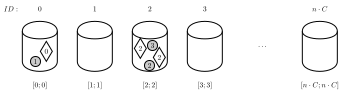
\includegraphics[width=\textwidth]{Appendix_I/GRAPH-VIZ-Example/a.pdf}
		\vspace{1em}
		\caption{}
		\label{fig:graphViz:b}
	\end{subfigure}
	\hfill\null
	\caption{
		Wygenerowana ilustracja grafu przez skrypt \textsc{makeGraphViz.bash}.
		\textbf{(a)}~Kod pośredni pomiędzy danymi wejściowymi w standardowym formacie \textsc{DIMACS Implementation Challenge} a finalnym rysunkiem. Kod pośredni jest zapisany w języku \textsc{DOT}.
		\textbf{(b)}~Rysunek grafu wygenerowany przez program \textsc{GraphViz}.
	}
	\label{fig:graphViz}
\end{figure}

\subsubsection{randDistance.pl}


Przy pomocy tego skryptu jest możliwa szybka zmiana długości ścieżek w~grafie bez ingerowania w~jego strukturę.
Program na wejściu oczekuje $4$ parametrów, gdzie kolejno nimi są:

\begin{itemize}
	\item minimalna waga, jaką po wykonaniu skryptu mogą mieć krawędzie w~zadanym grafie,
	\item największa możliwa waga dla krawędzi (obie wartości muszą być liczbami naturalnymi),
	\item plik wejściowy, definiujący graf (w przyjętym na początku formacie),
	\item nazwa pliku wyjściowego.
\end{itemize}

Przykładowe wywołanie skryptu:

\begin{lstlisting}[language=bash]
pcname@user:/Scripts$ perl randDistance.pl 1 2 testTMH.gr out.gr
\end{lstlisting}


\subsubsection{TMH\_GraphHelper}


Jest to, poza \textsc{TMH\_Examples} i~\textsc{TMH\_Library}, trzeci projekt w~obrębie całej biblioteki, mający na celu generowanie poprawnych plików wejściowych dla wszystkich wcześniej wymienionych skryptów oraz samej biblioteki.
Program został napisany w~języku \textsc{Java} i~oferuje możliwość wygenerowania prostych, skierowanych grafów bez cykli~--- tak zwanych $DAG$'ów (ang. \textit{Directed acyclic graph})~--- z~określoną liczbą wierzchołków oraz krawędzi.
Program umożliwia także wygenerowanie grafu na podstawie liczby węzłów oraz prawdopodobieństwa, z~jakim wszystkie wierzchołki w~grafie będą mieć krawędzie (im większe, tym graf będzie gęstszy).
Program korzysta z~bibliotek: \textsc{stdlib.jar} i~\textsc{algs4.jar}, napisanych przez Roberta Sedgewick'a i~Kevina Wayne'a\footnote{
	Wspomniane biblioteki są zbiorem rozwiązań prezentowanych w~książce~\cite{books/daglib/0029345}, dostępnych do pobrania na stronie internetowej: \url{http://algs4.cs.princeton.edu/home/} na licencji \textsc{GNU GPLv3}.
}.
Procesem budowania aplikacji zarządza \textsc{Apache Maven}.

Program oczekuje następujących parametrów:

\begin{lstlisting}[language=bash]
pcname@user:/TMH_GraphHelper$ java -jar GraphHelper.jar
	<liczba węzłów w grafie wyjściowym>
	<liczba łuków/prawdopodobieństwo>
	<najmniejszy koszt krawędzi>
	<największy koszt krawędzi>
	<nazwa pliku wyjściowego>
\end{lstlisting}

W~przypadku podania drugiego parametru jako liczby zmiennoprzecinkowej, program założy, że podane zostało prawdopodobieństwo.




\section{API biblioteki}




Główną częścią składową wyżej omawianych aspektów biblioteki \textsc{TMH} jest projekt \textsc{TMH\_Library}, który stanowi całość omawianej biblioteki~--- reszta programów ma za zadanie ułatwiać z~nią pracę.
Głównej struktury projektu nie będziemy tutaj przedstawiać, gdyż biblioteka udostępnia cały jej kod źródłowy.
Skupimy się za to na omówieniu kluczowej części każdej biblioteki tzn. interfejsu, który udostępnia ona użytkownikowi.



\subsection{Konfiguracja środowiska}



Przy licznych algorytmach, których implementacje znalazły się w~bibliotece, udostępnia ona maksymalnie uproszczone \textbf{API} (ang. \textit{Application Programming Interface}) by było ono przede wszystkim intuicyjne i~proste w~użyciu.
Aby omówić wszystkie możliwości konfiguracyjne, jakie udostępnia nam biblioteka, prześledzimy krok po kroku schemat wykorzystania jednego z~algorytmów wyszukiwania najkrótszych ścieżek.

Przy tak szerokim wachlarzu algorytmów, jakie udostępnia biblioteka, nie sposób jest zapewnić jednakowy dostęp do wszystkich z~nich.
Niektóre do poprawnego działania wymagają ręcznego podania parametrów, inne działają tylko na podstawie pliku z~definicją grafu.
Aby ujednolicić sposób wywołania każdej z~funkcji przyjęto założenie, że dla każdego algorytm niezbędne są następujące elementy:

\begin{itemize}
	\item Konfiguracja algorytmu~--- jest to zbiór uniwersalnych wartości, jakie mogą charakteryzować problem najkrótszych ścieżek.
	Jedynym wymaganym parametrem do utworzenia takiej konfiguracji jest plik wejściowy zawierający informację o~węzłach źródłowych, dla których chcemy wyliczyć najkrótsze ścieżki do wszystkich pozostałych wierzchołków (prawidłowy format takiego pliku omówiliśmy w~rozdziale \ref{sub:fileWithSourceList}):
	\begin{lstlisting}[style=customc]
TMHConfig* config = createTMHConfig("file.ss");
	\end{lstlisting}
	Interfejs biblioteki udostępnia szereg metod umożliwiających zmianę tak załadowanej konfiguracji:
	\begin{itemize}
		\item W~przypadku, gdy algorytm wymaga podania parametru przez użytkownika, możemy go w~takiej sytuacji albo:
		\begin{itemize}
			\item zdefiniować przed wywołaniem algorytmu:
			\begin{lstlisting}[style=customc]
TMHNodeData* param = malloc(sizeof(TMHNodeData));
param = 2;
setAllowInterrupt(config,false,param);
			\end{lstlisting}
			\item zmusić algorytm do samodzielnego wybrania parametru (w takiej sytuacji zostanie wybrana wartość optymalna, jeżeli dla danego algorytmu łatwo jest ją obliczyć):
			\begin{lstlisting}[style=customc]
TMHNodeData* param = NULL;
setAllowInterrupt(config,false,param);
			\end{lstlisting}
			\item lub podać żądany parametr w~chwili, gdy algorytm sam poprosi o~jego podanie (poprzez ustawienie drugiego parametru funkcji na \KwTrue):
			\begin{lstlisting}[style=customc]
TMHNodeData* param = NULL;
setAllowInterrupt(config,true,param);
			\end{lstlisting}
		\end{itemize}
	\item jeśli algorytm nie wymaga podawania parametrów, to ten zapis jest ignorowany. 
	\end{itemize}
	\item Możemy dodatkowo wymusić walidację konfiguracji (zostanie sprawdzona poprawność wczytanych danych z~pliku, który został podany na wejście):
	\begin{lstlisting}[style=customc]
setCheckConfig(config,true);
	\end{lstlisting}
	\item zmienić sposób organizacji grafu (np. spróbować posortować go topologicznie):
	\begin{lstlisting}[style=customc]
setGraphOrder(config,NONE);
	\end{lstlisting}
	\item wybrać sposób reprezentacji grafu wejściowego:
	\begin{lstlisting}[style=customc]
setGraphStruct(config,ADJACENCY\_LIST);
	\end{lstlisting}
	\item określić, który algorytm ma zostać wywołany do rozwiązania tak zdefiniowanego problemu:
	\begin{lstlisting}[style=customc]
setAlgorithm(config,alg);
	\end{lstlisting}
	\item Ścieżka do pliku z~definicją grafu (\textsc{path})~--- format pliku musi być zgodny z~przyjętym (\textsc{DIMACS Implementation Challenge})
\end{itemize}

Szczegóły, dotyczące możliwych wartości parametrów przyjmowanych dla każdej z~wymienionych funkcji można znaleźć w~dokumentacji technicznej biblioteki i~tutaj nie będą omawiane.
Wywołania wszystkich algorytmów które zostały zaimplementowane, można dodatkowo znaleźć w~projekcie \textsc{TMH\_Examples}.
Po spełnieniu powyższych wymagań, algorytm tworzy instancję problemu:

\begin{lstlisting}[style=customc]
ins = createTMHAlgorithmInstance(config,path);
\end{lstlisting}

Mając tę strukturę, możemy wykonać na niej następujące operacje:

\begin{itemize}
\item Rozpocząć wykonywanie właściwego algorytmu, który w~wyniku zwróci graf o~wierzchołkach mających ustalone najkrótsze ścieżki do zdefiniowanego źródła.
\begin{lstlisting}[style=customc]
runTMHAlgorithm(algorithm,ins);
\end{lstlisting}
Interpretacja wyników zależy już od użytkownika końcowego.
Biblioteka zapewnia możliwość odtworzenia najkrótszej ścieżki do źródła z~dowolnego węzła w~grafie, zaś reszta leży w~rękach programisty, który będzie wykorzystywał omawianą bibliotekę.
\item Zniszczyć instancję problemu poleceniem:
\begin{lstlisting}[style=customc]
destroyTMHAlgorithmInstancje(config->algorithm,ins,false);
\end{lstlisting}
gdzie wartość ostatniego parametru decyduje także, czy wraz z~nią ma zostać usunięta informacja o~przechowywanej konfiguracji (w przypadku ustawienia parametru na \KwFalse~będziemy mogli wykorzystać ją do uruchomienia następnych algorytmów dla tej samej konfiguracji).
\item Zniszczyć konfigurację:
\begin{lstlisting}[style=customc]
destroyTMHConfigInstance(config);
\end{lstlisting}
\end{itemize}



\subsection{Dziennik zdarzeń}



Dziennik zdarzeń jest to mechanizm pozwalający użytkownikowi na śledzenie działań każdego z~algorytmów i~dostosowanie liczby wyświetlanych informacji o~takim działaniu.
Do obsługi dziennika zdarzeń interfejs biblioteki udostępnia trzy metody:
\begin{lstlisting}[style=customc]
enableLog(TRACE,false);
disableLog();
enableSaveLog("logFile",true);
\end{lstlisting}
Pierwsza z~nich uruchamia zapisywanie zdarzeń, które mają miejsce podczas działania algorytmu.
Umożliwia ona także dostosowanie poziomu ich szczegółowości (np. \textsc{TRACE}, \textsc{DEBUG}, \textsc{INFO}, itd.) oraz zdecydowania, czy wybrany poziom ma być jedynym, który będzie wyświetlany (wtedy drugi parametr powinien być ustawiony na wartość \KwTrue).
W~przeciwnym przypadku będą wyświetlane wszystkie wydarzenia, których priorytet jest wyższy bądź równy aktualnie wybranemu.
Ostatnia metoda przekierowuje wszystkie tak powstałe zapisy do wskazanego przez użytkownika pliku.
Jednocześnie umożliwia wybór, czy ma w~nich być również zamieszczana informacja o~czasie zajścia danego zdarzenia.
Jeżeli zapisywanie takich zdarzeń pozostanie włączone, a~nie zdecydujemy się na przekierowanie ich do pliku, to będą one wyświetlane na standardowe wyjście terminala razem z~innymi informacjami, które zdefiniuje użytkownik (z poziomu $API$ nie ma możliwości samodzielnego definiowania zdarzeń).
W~następnym rozdziale został przedstawiony pełen zapis wydarzeń, jakie miały miejsce podczas pracy jednego z~podstawowych algorytmów wyszukujących najkrótsze ścieżki).

\newpage



\section{Przykładowa sesja}




\tiny
\begin{lstlisting}[mathescape,language=bash]
22:16:21 | INFO | [TMHIOHelper] Open data file: '/home/tomasz/workspace/TMH_Tests/ss/test.ss'.
22:16:21 | INFO | [TMHIOHelper] Loading auxiliary data for problem: 'Shortest Path Problem':
	Targeted algorithm mode		:	ss
	Number of definitions to read	:	1
22:16:21 | INFO | [TMHIOHelper] Auxiliary definition added:
	Find all paths from node:	1
22:16:21 | INFO | [TMHIOHelper] Open data file: '/home/tomasz/workspace/TMH_Tests/gr/testTMH1.gr'.
22:16:21 | INFO | [TMHIOHelper] Loading data for problem: 'Shortest Path Problem':
	Number of nodes	:	5
	Number of arcs	:	7
22:16:21 | INFO | [TMHIOHelper] Arc definition read:
	1		---(6)--->		2
...........................................................
22:16:21 | INFO | [TMHIOHelper] Arc definition read:
	5		---(6)--->		4
22:16:21 | INFO | [DKQD] PreExecution summary:
	Running algorithm	:	Dijkstra's Naive Implementation with double-linked lists
	Selected mode		:	Single Source
	Source node's ID	:	1
22:16:21 | TRACE | [DKQD] Initializing graph with 5 nodes.
Set node with ID: 1 as a source node with distanceLabel = 0.
22:16:21 | TRACE | [DKQD] Initialize double-linked list with source node with ID: 1 (distance: 0).
22:16:21 | TRACE | [DKQD] Query for next element from queue.
22:16:21 | TRACE | [DKQD] Queried node details:
	Node ID		:	1
	Distance	:	0
	Parent's ID	:	no parent
22:16:21 | TRACE | [DKQD] Checking arc:	1	---(6)--->	3
	Target's distance labels:
		Old	:	$ \infty $
		New	:	6
22:16:21 | TRACE | [DKQD] Executing relaxation. Changing nodes' linkage from:
	No parents found for node with ID: 3 ($ \infty $)
to:
	1 (0)	---(6)--->	3 (6)
22:16:21 | TRACE | [DKQD] Checking arc:	1	---(6)--->	2
	Target's distance labels:
		Old	:	$ \infty $
		New	:	6
22:16:21 | TRACE | [DKQD] Executing relaxation. Changing nodes' linkage from:
	No parents found for node with ID: 2 ($ \infty $)
to:
	1 (0)	---(6)--->	2 (6)
22:16:21 | TRACE | [DKQD] Query for next element from queue.
22:16:21 | TRACE | [DKQD] Queried node details:
	Node ID		:	2
	Distance	:	6
	Parent's ID:	:	1
22:16:21 | TRACE | [DKQD] Checking arc:	2	---(5)--->	5
	Target's distance labels:
		Old	:	$ \infty $
		New	:	11
22:16:21 | TRACE | [DKQD] Executing relaxation. Changing nodes' linkage from:
	No parents found for node with ID: 5 ($ \infty $)
to:
	2 (6)	---(5)--->	5 (11)

22:16:21 | TRACE | [DKQD] Checking arc:	2	---(6)--->	4
	Target's distance labels:
		Old	:	$ \infty $
		New	:	12
22:16:21 | TRACE | [DKQD] Executing relaxation. Changing nodes' linkage from:
	No parents found for node with ID: 4 ($ \infty $)
to:
	2 (6)	---(6)--->	4 (12)
22:16:21 | TRACE | [DKQD] Checking arc:	2	---(6)--->	3
	Target's distance labels:
		Old	:	6
		New	:	12
22:16:21 | TRACE | [DKQD] Query for next element from queue.
22:16:21 | TRACE | [DKQD] Queried node details:
	Node ID		:	3
	Distance	:	6
	Parent's ID:	:	1
22:16:21 | TRACE | [DKQD] Checking arc:	3	---(6)--->	5
	Target's distance labels:
		Old	:	11
		New	:	12
22:16:21 | TRACE | [DKQD] Query for next element from queue.
22:16:21 | TRACE | [DKQD] Queried node details:
	Node ID		:	5
	Distance	:	11
	Parent's ID:	:	2
22:16:21 | TRACE | [DKQD] Checking arc:	5	---(6)--->	4
	Target's distance labels:
		Old	:	12
		New	:	17
22:16:21 | TRACE | [DKQD] Query for next element from queue.
22:16:21 | TRACE | [DKQD] Queried node details:
	Node ID		:	4
	Distance	:	12
	Parent's ID:	:	2
22:16:21 | TRACE | [DKQD] Queried node with ID: 4 has no outgoing arcs.
\end{lstlisting}
\normalsize